\section{Problem Set 2}
\subsection{Everything is Relative}

\subsubsection{Variations in Initial Orbital Elements} \label{sec:rel_init_oe}
We will use the initial quasi-nonsingular relative orbital elements (ROE) given in section \ref{sec:ROE_init}, except with zero difference in semi-major axis ($\delta a =0$). Using the chief's initial quasi-nonsingular absolute orbital elements, we can find the initial absolute orbital elements and then the initial position and velocity in ECI of both of the deputy satellites (SV2 and SV3), through the following method: 

The subscript $o$ indicates the chief or "observer", while the subscript $t$ indicates the deputy or "target". First, we convert the chief semi-major axis from km to m to agree with the units of the ROEs:
\begin{align}
   a_o \leftarrow a_o \cdot 10^3 
\end{align}


Then, we compute the deputy semi-major axis, eccentricity components, inclination, RAAN, and argument of latitude:
    \begin{align}
    a_t &= \frac{a_o + d_a}{10^3} \\
    e_{x,t} &= \frac{d_{e_x}}{a_o} + e_{x,o} \\
    e_{y,t} &= \frac{d_{e_y}}{a_o} + e_{y,o} \\
    i_t &= \frac{d_{i_x}}{a_o}  + i_o \\
    \Omega_t &= \frac{d_{i_y}}{a_o \cdot \sin(i_o)}  + \Omega_o \\
    u_t &=  \frac{d_\lambda}{a_o}+ u_o - (\Omega_t - \Omega_o) \cdot \cos(i_o)
\end{align}


Then the quasi-nonsingular orbital elements can be converted to the Keplerian orbital elements through the method outlined in section \ref{sec:initial_oe}. Finally, the Keplerian orbital elements can be converted to position and velocity in the ECI frame through the method outlined in section \ref{sec:initial_ECI}. This results in the initial ECI position and velocity of both the deputies: 

\begin{align}
    \mathbf{r}_{\text{SV2}} &=
    \begin{bmatrix}
    -3574.8655 \\
    -2953.8783 \\
    -5180.4446
    \end{bmatrix} \text{km} \\
    \mathbf{v}_{\text{SV2}} &=
    \begin{bmatrix}
    -5.3901 \\
    -2.0500 \\
    \phantom{-}4.8991
    \end{bmatrix} \text{km/s} \\
    \mathbf{r}_{\text{SV3}} &=
    \begin{bmatrix}
    -3606.2292 \\
    -2965.3946 \\
    -5150.6778
    \end{bmatrix} \text{km} \\
    \mathbf{v}_{\text{SV3}} &=
    \begin{bmatrix}
    -5.3652 \\
    -2.0292 \\
    \phantom{-}4.9357
    \end{bmatrix} \text{km/s}
\end{align}

\subsubsection{Numerical Integration of Non-linear Equations for Relative Motion} \label{sec:nonlinear_rel_eom}
Given the initial ECI conditions of the chief (SV1) and the deputies (SV2 and SV3), we can find the initial position and velocity of the deputies in the RTN frame of the chief. Similar to what was shown in Equations \ref{eq:eci2rtn} to \ref{eq:v_rtn}, the rotation matrix from ECI to RTN is done as follows, 

\begin{align}
    \boldsymbol{\hat{R}} &= \frac{\boldsymbol{r}^{ECI}_{SV1}}{||\boldsymbol{r}^{ECI}_{SV1}||} \\ \label{eq:q_eci2rtn_rel}
    \boldsymbol{\hat{N}} &= \frac{\boldsymbol{r}^{ECI}_{SV1} \times \boldsymbol{v}^{ECI}_{SV1}}{||\boldsymbol{r}^{ECI}_{SV1} \times \boldsymbol{v}^{ECI}_{SV1}||} \\
    \boldsymbol{\hat{T}} &= \boldsymbol{\hat{N}} \times \boldsymbol{\hat{R}} \\
    Q_{eci2rtn} &= \begin{bmatrix}
        \boldsymbol{\hat{R}} & \boldsymbol{\hat{T}} & \boldsymbol{\hat{N}}
    \end{bmatrix}^T
\end{align}

We take $\boldsymbol{\rho}$ as the relative position between the chief and deputy (for the equations below, we use SV2), so $\boldsymbol{\rho}^{RTN}$ is relative position of the deputy in the chief's RTN frame. Similarly, $\boldsymbol{\dot{\rho}}^{RTN}$ is the relative velocity of the deputy in the chief's RTN frame.

\begin{align}
    \boldsymbol{\rho}_{SV2}^{ECI} &= \boldsymbol{r}^{ECI}_{SV2} - \boldsymbol{r}^{ECI}_{SV1}\\
    \boldsymbol{r}^{RTN}_{SV1} &= Q_{eci2rtn} \boldsymbol{\rho}_{SV2}^{ECI} \\
    \boldsymbol{\dot{\rho}}^{RTN}_{SV2} &= Q_{eci2rtn} \left(\boldsymbol{v}^{ECI}_{SV2} - \boldsymbol{v}^{ECI}_{SV1}\right)  - \omega_{RTN} \times \boldsymbol{\rho}^{RTN}_{SV2} \label{eq:v_rtn_rel}
\end{align}

where $\omega_{RTN} = \begin{bmatrix}
    0 & 0 & ||r\times v ||/||r||^2
\end{bmatrix}$. We can define $\boldsymbol{\rho}^{RTN}$ and $\boldsymbol{\dot{\rho}}^{RTN}$ (Here, the time derivative accounts for the rotating RTN frame) to be

\begin{align}
    \boldsymbol{\rho}^{RTN} &= \begin{bmatrix}
        x & y & z
    \end{bmatrix}^T, \\
    \boldsymbol{\dot{\rho}}^{RTN} &= \begin{bmatrix}
        \dot{x} & \dot{y} & \dot{z}
    \end{bmatrix}^T 
\end{align}

The non-linear equations of motion for relative motion give us a method to numerically propagate $x, y, \text{and} \ z$. The equations of motion are given by

\begin{align}
\ddot{x} &= 2\dot{\theta}_0 \dot{y} + \ddot{\theta}_0 y - \dot{\theta}_0^2 x -\frac{\mu (r_0 + x)}{\left[(r_0 + x)^2 + y^2 + z^2\right]^{3/2}} + \frac{\mu}{r_0^2} \\
\ddot{y} &= - 2\dot{\theta}_0 \dot{x} - \ddot{\theta}_0 x + \dot{\theta}_0^2 y  -\frac{\mu y}{\left[(r_0 + x)^2 + y^2 + z^2\right]^{3/2}} \\
\ddot{z} &= -\frac{\mu z}{\left[(r_0 + x)^2 + y^2 + z^2\right]^{3/2}}
\end{align}

The value $r_0$ is the radial position of the chief when expressed in the RTN frame (or, the norm of the position vector of the chief) $\boldsymbol{r}_0 = ||\boldsymbol{r}^{ECI}_{SV1}|| = \boldsymbol{r}^{RTN}_{SV1, x}$ 
Here, $\dot{\theta}$ is the angular velocity of the chief (and thus the angular velocity of the RTN frame), and $\ddot{\theta}$ is the angular acceleration of the chief. We can get 
\begin{align}
    \dot{\theta} &= \frac{{||\boldsymbol{r}_{SV1}^{ECI} \times \boldsymbol{v}_{SV1}^{ECI}||}}{r_0^2} \\
    \ddot{\theta} &= -\frac{2\dot{r}_0\dot{\theta}}{r_0}
\end{align}

Here, $\dot{r}_0$ is the rate of change in the length of the position vector of the chief. A convenient way to get this is to take the radial component of the chief's velocity in its RTN frame.

\begin{align}
    \dot{r}_0 = \boldsymbol{v}^{RTN}_{SV2, x}
\end{align}

With these differential equations and the initial conditions in RTN, the relative motion of the deputy satellites is propagated using RK4 (Runga-Kutta-4) through the entire duration that the chief is propagated. The specifications of the time-steps are the same as Equation \ref{eq:timestep}.

All the above operations are also repeated for the third satellite, SV3/Docker, for which the initial conditions are given in Section \ref{sec:rel_init_oe}.
The results of the propagation are shown in Figures \ref{fig:rel_3d_traj}, \ref{fig:rel_3d_proj}, \ref{fig:rel_pos_vel_rtn_sv2}, and \ref{fig:rel_pos_vel_rtn_sv3}.

\subsubsection{Computing Relative Orbits using FODE of Absolute Motion}

In this method, we perform the absolute orbit propagation of the three satellites SV1, SV2, and SV3 using just the fundamental orbital differential equations of absolute motion utilized in Section \ref{sec:fode_simulation}. Once the motion of all three satellites is calculated, the positions and velocities of the deputies SV2 and SV3 can be converted into the RTN frame of the chief using the procedure described in Section \ref{sec:nonlinear_rel_eom} in equations \ref{eq:q_eci2rtn_rel} to \ref{eq:v_rtn_rel}. This FODE propagation is done with the same numerical method (RK4) and time-steps as the nonlinear relative motion method, given in equation \ref{eq:timestep}. The results of this method are shown and compared in Figures \ref{fig:rel_3d_traj}, \ref{fig:rel_3d_proj}, \ref{fig:rel_pos_vel_rtn_sv2}, and \ref{fig:rel_pos_vel_rtn_sv3}.

It is interesting to note that in Figure \ref{fig:rel_3d_traj}, the relative orbits are not centered around the $x = 0$ point. Instead, the deputy satellites always have a negative radial position despite having the same semi-major axis as the chief. This is because we are using rectilinear co-ordinates instead of curvi-linear co-ordinates, and so these plots don't correct for the curvature of the earth, which is non-negligible when one has large cross-track separations.

\begin{figure}[H]
    \centering
    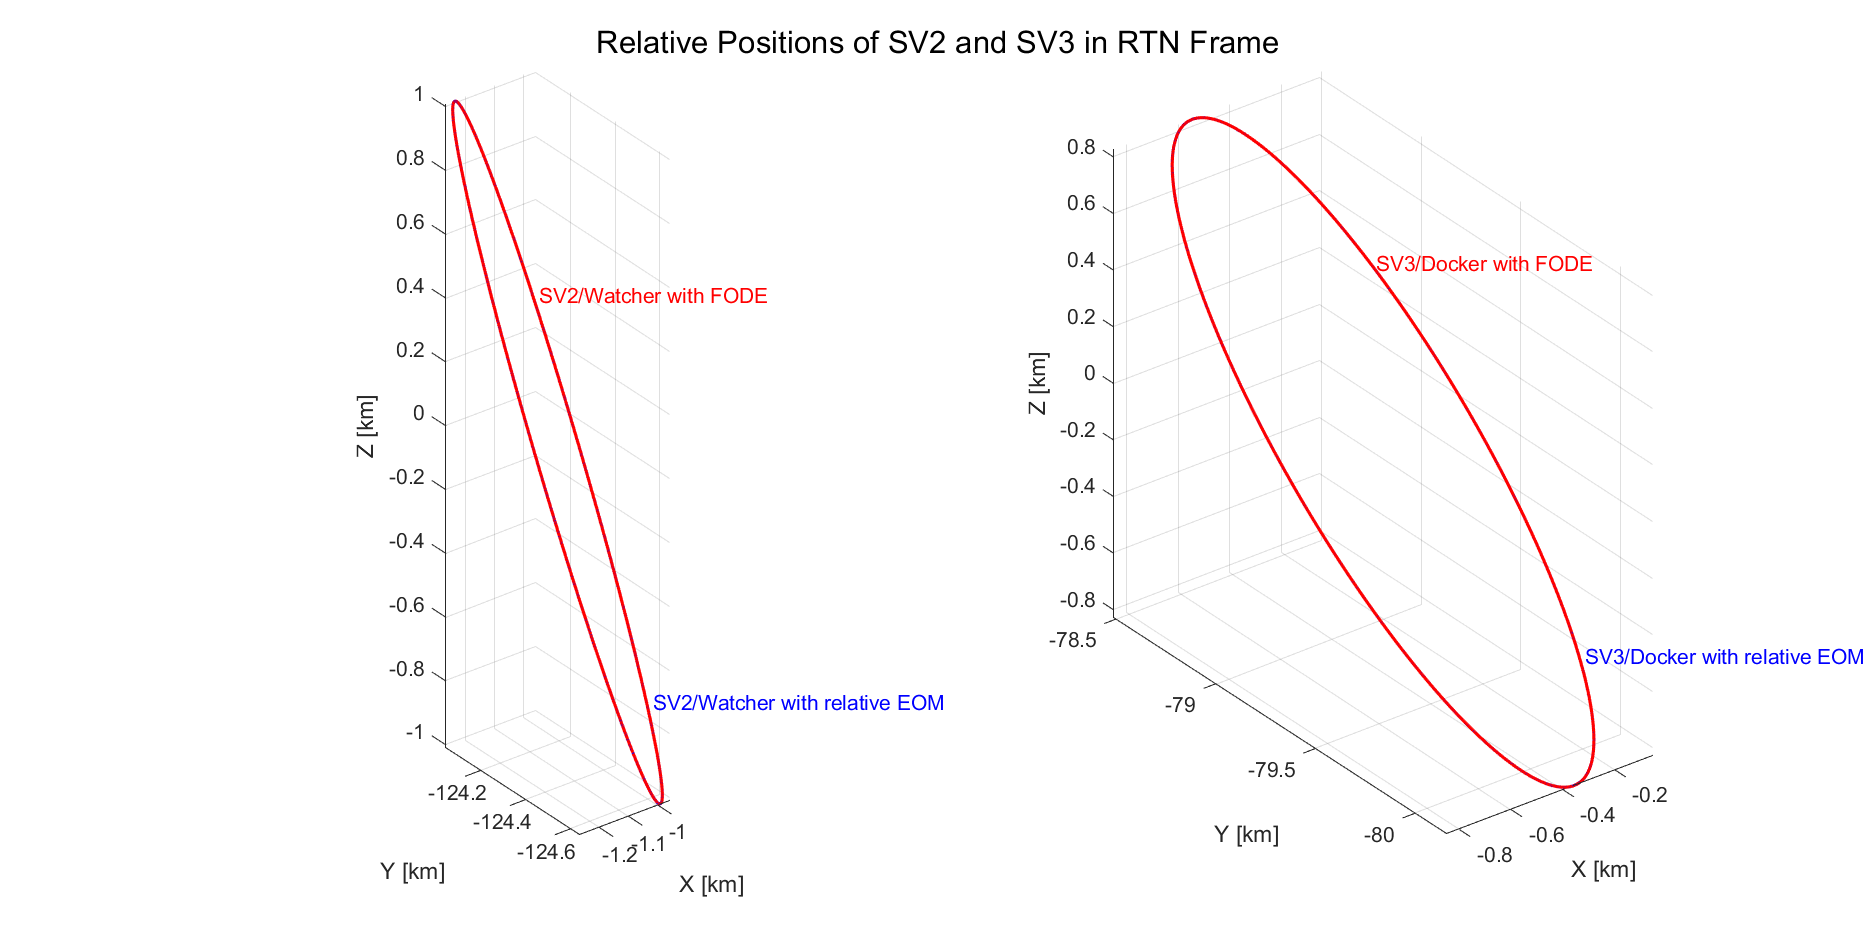
\includegraphics[width=0.9\linewidth]{sim/figures/SV2_SV3_3d_traj_rel.png}
    \caption{The 3D trajectories of SV2 and SV3 with the relative orbit propagation and FODE absolute motion propagation}
    \label{fig:rel_3d_traj}
\end{figure}

\begin{figure}[H]
    \centering
    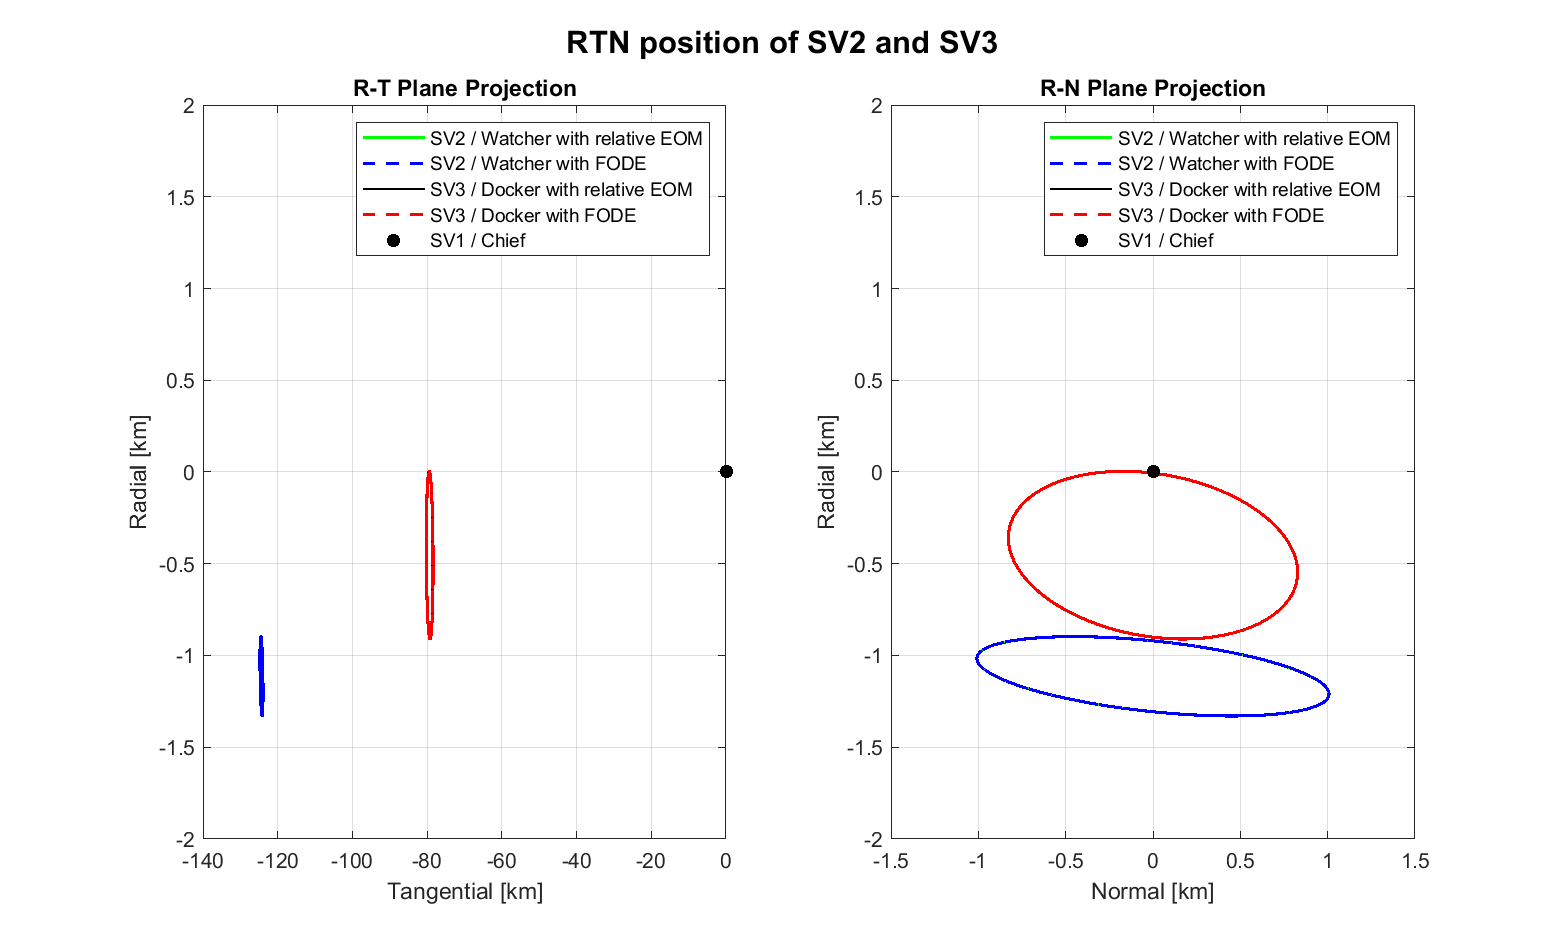
\includegraphics[width=0.9\linewidth]{sim/figures/RTN_projection.png}
    \caption{Projection of the trajectory to the Radial-Tangential and Radial-Normal planes, for both SV2 and SV3, and for both methods.}
    \label{fig:rel_3d_proj}
\end{figure}

\begin{figure}[H]
    \centering
    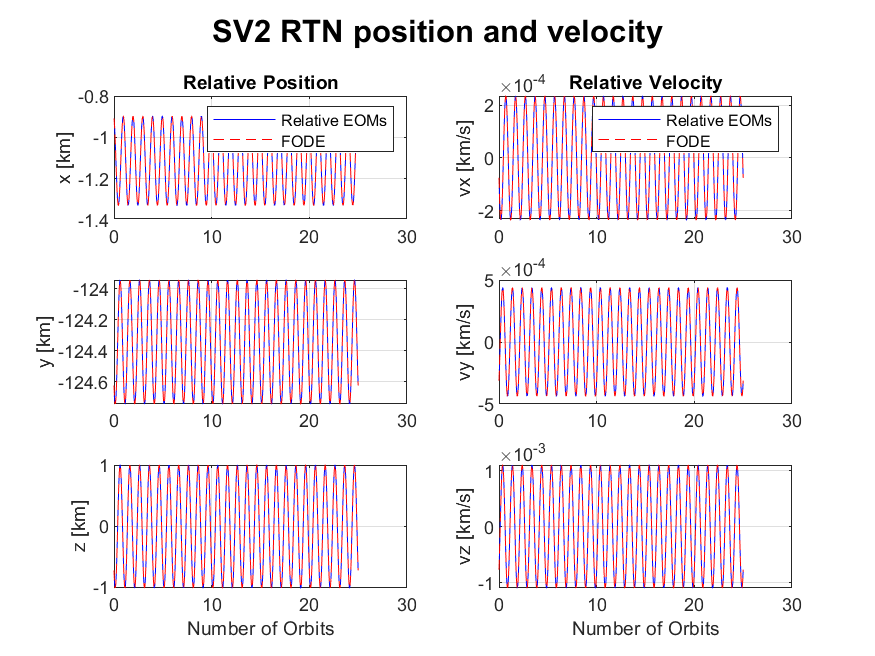
\includegraphics[width=0.7\linewidth]{sim/figures/SV2_rel_pos_vel.png}
    \caption{The RTN position and velocity of SV2, for both methods of relative orbit calculation.}
    \label{fig:rel_pos_vel_rtn_sv2}
\end{figure}

\begin{figure}[H]
    \centering
    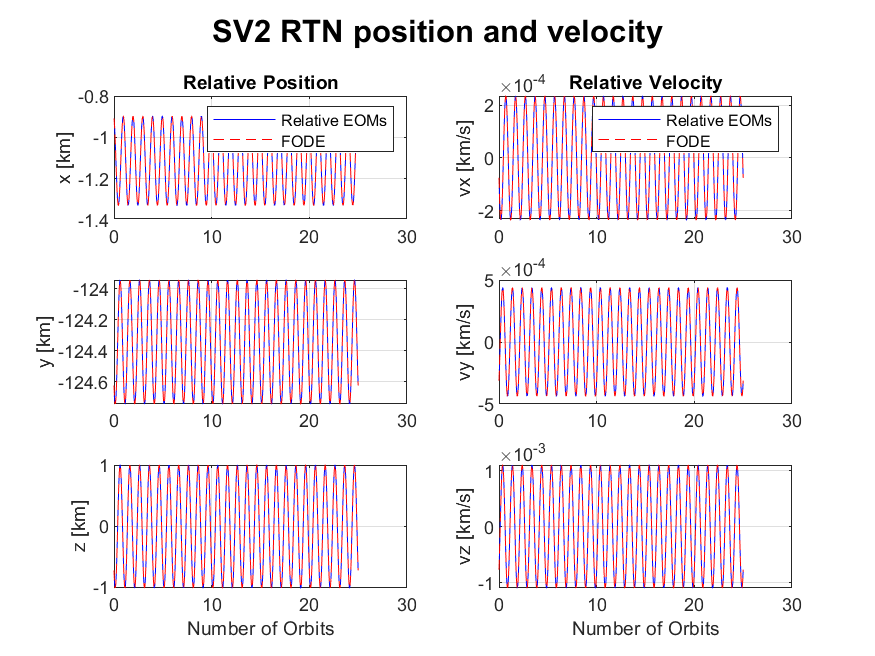
\includegraphics[width=0.7\linewidth]{sim/figures/SV2_rel_pos_vel.png}
    \caption{The RTN position and velocity of SV3, for both methods of relative orbit calculation.}
    \label{fig:rel_pos_vel_rtn_sv3}
\end{figure}

\subsubsection{Comparison of Relative Orbit Calculation Methods}
Since the two methods used above for relative orbit calculation are mathematically equivalent irrespective of initial conditions utilized, the only difference in the results should be numerical errors. Figures \ref{fig:error_in_SV2_rel} and \ref{fig:error_in_SV3_rel} showcase the error between the two methods for SV2 and SV3 respectively.

\begin{figure}
    \centering
    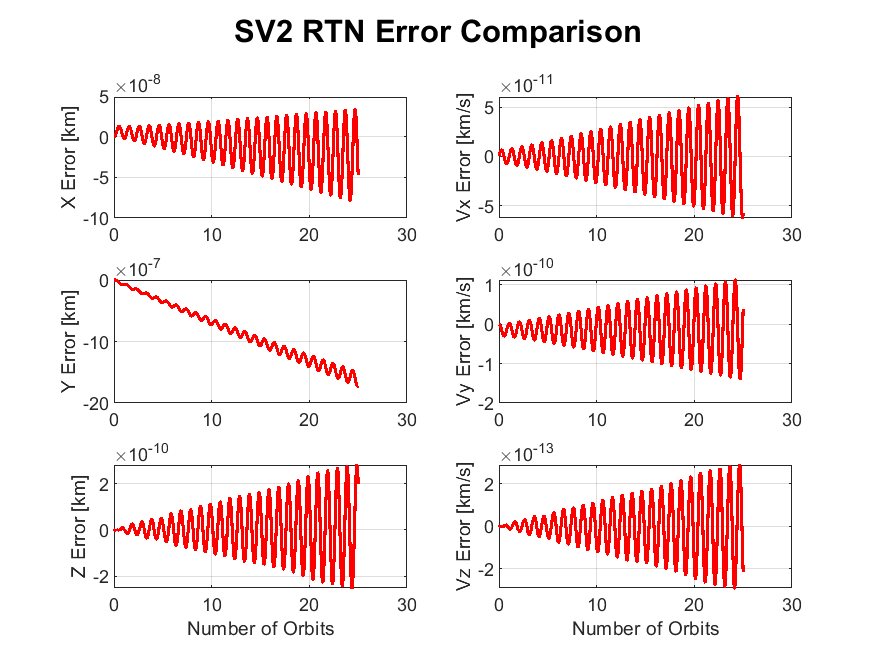
\includegraphics[width=0.75\linewidth]{sim/figures/SV2_error_in_rel_methods.png}
    \caption{Error between the relative orbits of SV2 calculated by FODE methods and Nonlinear relative EOM methods.}
    \label{fig:error_in_SV2_rel}
\end{figure}

\begin{figure}
    \centering
    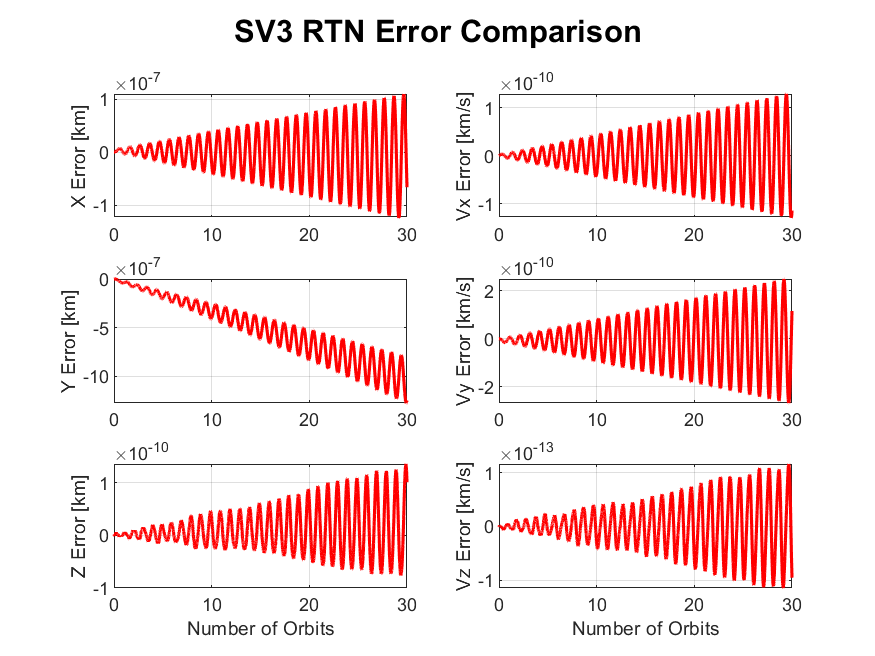
\includegraphics[width=0.75\linewidth]{sim/figures/SV3_error_in_rel_methods.png}
    \caption{Error between the relative orbits of SV3 calculated by FODE methods and Nonlinear relative EOM methods.}
    \label{fig:error_in_SV3_rel}
\end{figure}

We see that using fine time-steps, we can keep the numerical error between the two methods contained to negligible amounts.

This also holds when the initial condition has a semi-major axis difference, which we can see in Figure \ref{fig:error_in_SV2_rel_nonzero_a} for SV2 when its initial conditions of SV2 have a non-zero difference in the semi-major axis. Although the error has a different profile than in the previous plots, the error is still at a much smaller magnitude than the actual values, so is negligible, and can be attributed to numerical error.

\begin{figure}
    \centering
    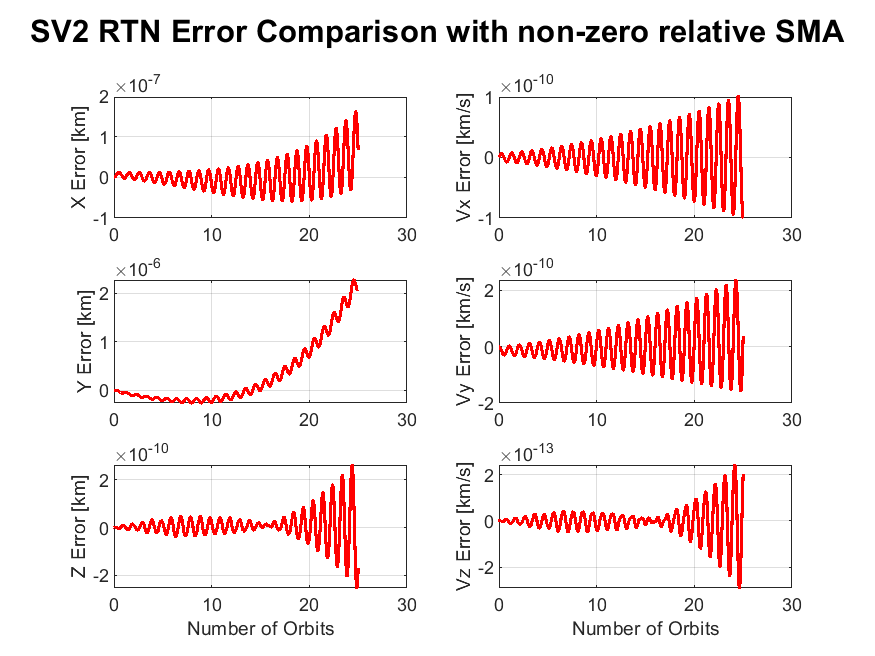
\includegraphics[width=0.7\linewidth]{sim/figures/SV2_error_in_rel_methods_nonzero_a.png}
    \caption{Error between the relative orbits of SV2 calculated by FODE methods and Nonlinear relative EOM methods, in a case where there is a relative semi-major axis difference.}
    \label{fig:error_in_SV2_rel_nonzero_a}
\end{figure}

\subsubsection{Derivation of Impulsive Maneuver for Bounded Period Motion}
To re-establish a bounded periodic relative motion between the deputy and the chief, the specific mechanical energies and, thus, the semi-major axes of the orbits must match. For a circular chief orbit (or near-circular as in our case), an equilibrium continuum exists that satisfies the energy matching condition: when the deputy is co-located on the same circular orbit of the chief. To achieve this condition, the semi-major axis of the deputy must be the same as the chief's, leading to both having the same mean motion. Therefore, an impulsive maneuver to adjust the deputy's semi-major axis is chosen. The Gauss Variational Equation (GVE) for semi-major axis is given as follows:
\begin{align}
\frac{da}{dt} &= \frac{2e \sin f}{n \sqrt{1 - e^2}} f_r + \frac{2a \sqrt{1 - e^2}}{n r} f_t
\end{align}
In order to find the size (delta-v) and location of the maneuver, we can integrate the GVE over an impulsive maneuver delta-v with constant orbit elements, using the following framework:
\begin{align}
\int_{t^-}^{t^+} \frac{d\vec{o}}{dt} dt &= \int_{t^-}^{t^+} \frac{\partial \vec{o}}{\partial \vec{v}} \left( \vec{a} \right) dt
\end{align}
Applying this to the semi-major axis GVE results in the following:
\begin{align}
\Delta a = \int \frac{da}{dt} dt = \int \left( \frac{2a \sqrt{1 - e^2}}{n r} \cdot f_t \right) dt
\end{align}
And then assuming impulsive maneuver, \( \int f_t dt = \Delta v_t \):
\begin{align}
\Delta a = \frac{2a \sqrt{1 - e^2}}{n r} \Delta v_t
\end{align}
Rearranging for $\Delta v_t$:
\begin{align}
\Delta v_t = \frac{n r}{2a \sqrt{1 - e^2}} \Delta a
\end{align}
This can be simplified for near-circular orbits \( e = 0, a \approx r \), however we will use the more accurate previous expresision:
\begin{align}
\Delta v_t = \frac{n}{2} \Delta a
\end{align}

Note that we ignore the radial component of the GVE because radial acceleration is not as efficient at changing \( a \) as tangential acceleration is. Also, the radial term only contributes if \( e \neq 0 \), and the maneuver does not occur at periapsis or apoapsis due to its dependence on true anomaly \(\sin f\). While there is some eccentricity, the second condition will not hold for our maneuver. Thus, the most fuel-efficient maneuver will be in the along-track direction.

For the most fuel-efficient location, the impulsive maneuver should be applied at periapsis due to the Oberth effect. Note that this is assuming the relative phasing of the deputy from the chief is less important than fuel efficiency. Also note that if the orbit is near-circular, there is not much added efficiency by performing at the periapsis as compared to anywhere else due to very small velocity changes throughout the orbit.

Therefore, the most fuel-efficient impulsive maneuver will be performed at the periapsis of the deputy's orbit in the along-track direction with size $\Delta v_t$. A single-burn maneuver will lead to a change in the eccentricity, which is acceptable for our purposes in this case. If no eccentricity change was desired, this could be accomplished with splitting up the single maneuver into two burns with one at the periapsis and one at the apoapsis, each with half of the original delta-v. 

\subsubsection{Application of Impulsive Maneuver for Bounded Period Motion}
To apply the impulsive maneuver to re-establish bounded periodic motion, we first found the required $\Delta v_t$ from the desired $\Delta a$ to match the chief's semi-major axis. The differences in semi-major axes of the deputies were arbitrarily set to be large to create a noticeable drift. Specifically, the initial conditions were:

\begin{align*}
\delta a_{\text{SV2, init}} &= 200 \text{ m} \\
\delta a_{\text{SV3, init}}  &= -1000 \text{ m}
\end{align*}

Both orbits were propagated for approximately 12 orbits. Then burn was performed at the periapsis of the 12th orbit for fuel-optimality. As seen in both Figure \ref{fig:SV2_rel_pos_vel_eom_maneuver} and \ref{fig:SV3_rel_pos_vel_eom_maneuver}, the drift in radial ($x$) and tangential ($y$) positions was stopped by the maneuver. Instead of oscillations with secular drift, there are now purely oscillations post-maneuver. The secular drift arises from differences in the mean motions of the deputy and chief due to the difference in semi-major axis of the two. The drift cancellation arises from the equilibrium condition of semi-major axis matching. The amplitude of oscillations is related to the phasing of the deputies with respect to the chief, which is a function of timing and relative positioning during the maneuver. Note that while the changes in relative position appear to be instantaneous, they occur over a short period of time. The magnitude of these changes arises from the arbitrary initial conditions set and the amount of drift before the maneuver is applied. 

\begin{figure}[H]
    \centering
    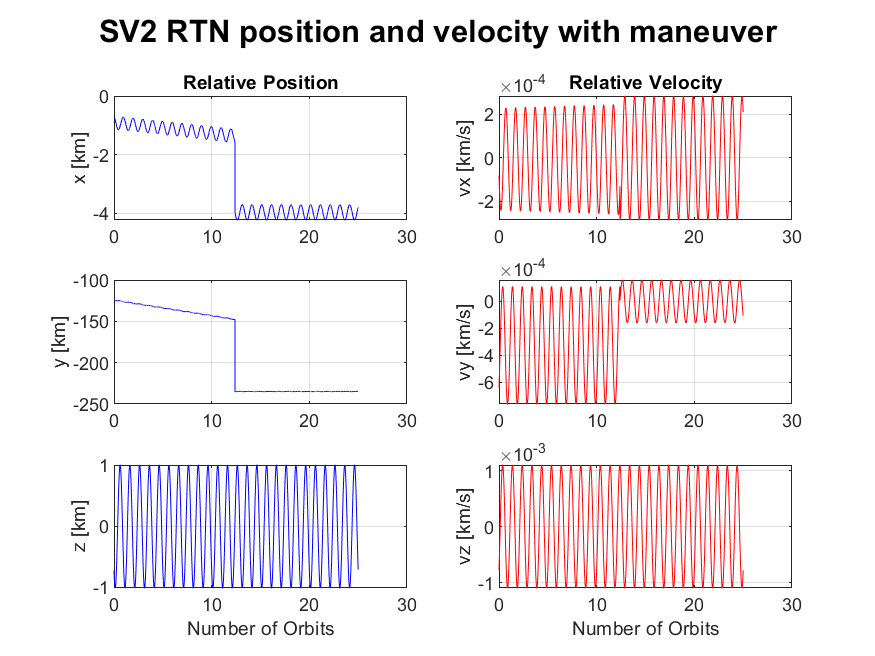
\includegraphics[width=0.7\linewidth]{sim/figures/SV2_rel_pos_vel_eom_maneuver.png}
    \caption{SV2 RTN position and velocity with maneuver applied}
    \label{fig:SV2_rel_pos_vel_eom_maneuver}
\end{figure}

\begin{figure}[H]
    \centering
    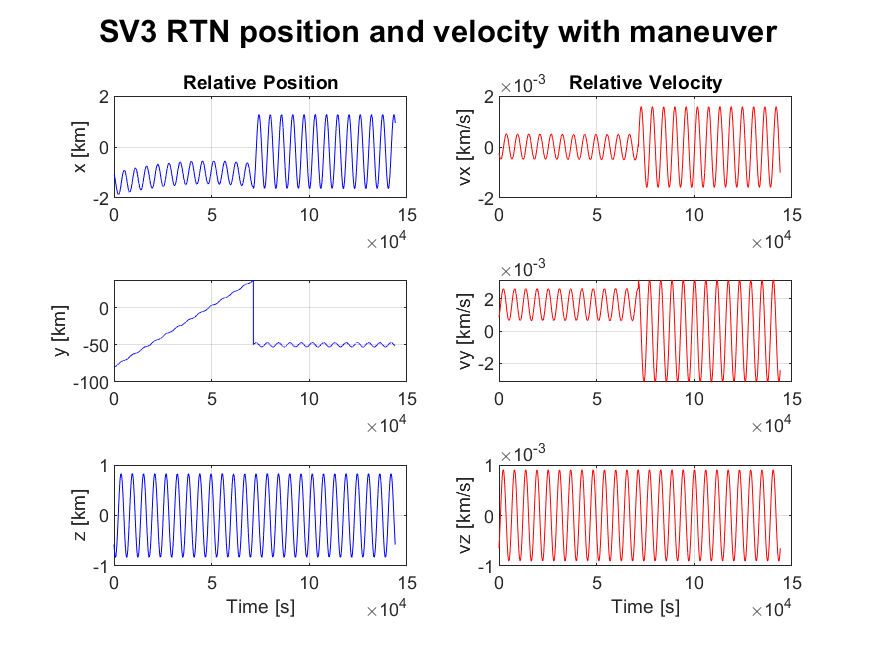
\includegraphics[width=0.7\linewidth]{sim/figures/SV3_rel_pos_vel_eom_maneuver.png}
    \caption{SV3 RTN position and velocity with maneuver applied}
    \label{fig:SV3_rel_pos_vel_eom_maneuver}
\end{figure}